\documentclass[hyperref={pdfpagemode=FullScreen},9pt]{beamer}

\usetheme{Warsaw}
\usepackage[latin1]{inputenc}
\usepackage[T1]{fontenc}

%\usepackage[frenchb]{babel}
%
% Packages pour le français
%\usepackage[T1]{fontenc} 
%\usepackage[utf8]{inputenc}
%\usepackage[frenchb]{babel}
%
% pour un pdf lisible à l'écran
% il y a d'autres choix possibles 
%\usepackage{pslatex}
%\usepackage{times}
%\usepackage{ifthen}
%\usepackage{array}
%\usepackage{layout}
%\usepackage{tabularx}
%\usepackage{supertabular}
%\usepackage{setspace}
%\usepackage{lmodern}
\usepackage{graphicx}
\usepackage{amsfonts}
\usepackage{amsmath}
%\usepackage{mathrsfs}
%\usepackage{algorithmic}
\usepackage{algorithmicx}
\usepackage{algorithm}
\usepackage{algpseudocode}
\usepackage{algpascal}
\usepackage{algc}
%\usepackage{multimedia}
%\usepackage{animate}
\usepackage{hyperref}
\usepackage{cases}
%\usepackage{pgf,pgfarrows,pgfnodes,pgfautomata,pgfheaps,pgfshade}
\usepackage{amsmath,amssymb}
\usepackage[latin1]{inputenc}
%\usepackage{colortbl}
\usepackage[english]{babel}
%\usepackage{subfigure}
\usepackage{epsfig,graphics}


%\usepackage[frenchb]{babel}
%\usepackage{aeguill}
%\usepackage{amsmath,amsthm,multirow}
%\usepackage{hyperref}
\usepackage{color}
\usepackage{multimedia}
%\def\ds{\displaystyle}
%\usepackage{amssymb}


\usepackage{tikz}
\usetikzlibrary{arrows}
\usetikzlibrary{snakes}
\usetikzlibrary{shapes}
\usetikzlibrary{backgrounds}

	
\newcommand\R{\mathbb{R}}
\newcommand\C{\mathbb{C}}
\newcommand\D{\mathscr{D}}
\newcommand\T{\mathbb{T}}
\newcommand\N{\mathbb{N}}
\newcommand\Z{\mathbb{Z}}
\newcommand\Q{\mathbb{Q}}
\newcommand\Ng[1]{\left| #1 \right|_{\gamma}}
\newcommand\Ngs[2]{\left| #1 \right|_{\gamma^{#2}}}
\newcommand\Hg{H_{\gamma}(\R)}
\newcommand\Hgs[1]{H_{\gamma^{#1}}(\R)}
\newcommand\Nb[1]{\left| #1 \right|_{\beta}}
\newcommand\Hb{H_{\beta}(\R)}
\newcommand\Inf{{\mbox Inf}}
\newcommand\Min{{\mbox Min}}
\newcommand\Lg{\mathscr{L}_{\gamma}}
%\newcommand\inf{\mbox{Inf}}
 
% Desactiver symbole d'en bas à droite 
\setbeamertemplate{navigation symbols}{}
	
%\setbeamercolor{block title}{fg=red,bg=black!5}	

% pour le style et couleurs
%\usetheme{CambridgeUS}%{Goettingen}
%\usecolortheme{orchid}
%\usefonttheme{nom du theme de police}
%\useinnertheme{nom du theme interne}
%\useoutertheme{smoothbars}
%

%Automatiser le sommaire au début de chaque section
%\AtBeginSection[]{
%  \begin{frame}{Sommaire}
%  \small \tableofcontents[currentsection, hideothersubsections]
%  \end{frame} 
%}


 \newcommand{\Frac}[2] {\frac{\textstyle #1} {\textstyle #2}}
%\newcommand{\lot}{|\hspace{-1.5pt}\backslash}
\font\Blackbrd=msbm10 scaled 1200       % Font for text
\font\Blackbrdsub=msbm10 scaled 900     % Font for index



\title{Stabilized Time Schemes for nonlinear parabolic equations}



\author{J-P. CHEHAB\inst{1}}


\institute{
  \inst{1}
  LAMFA, UMR 7352, Universit\'e de Picardie Jules Verne, Amiens, France
(jean-paul.chehab@u-picardie.fr)\\

  }
%\logo{\includegraphics[height=1.0cm]{logo2_lamav.eps}}
\centerline{(Joint work with M. Brachet (Univ. Lorraine at Metz))}
\date{NL2A, CIRM, October 24-28, 2016}
%%%%%%%%%%%%%%%%
\begin{document}

\frame{\titlepage}

\begin{frame}<beamer>
\frametitle{Outline}
\tableofcontents
\end{frame}


\section{Motivation}
\begin{frame}[label=introduction]
	\frametitle{Motivation}
	Consider the dynamical system (obtained after discretization in space)
	\begin{equation}
\begin{array}{l}
\Frac{du}{dt} +Au=f,\\
u(0)=u_0,
\end{array}
\end{equation}
$A$ : stiffness matrix (SPD)
\pause
	\begin{block}{Classical antagonism}
	\begin{itemize}
	\item Explicit time schemes (such as Forward Euler''s) produce fast iterations but suffer from hard time step restriction
	$$
	0<\Delta t <\Frac{2}{\rho(A)}
	$$
\pause
	\item Implicit time schemes (such as Backward Euler's) are stable but need to solve a linear system at each step, sometimes with a full matrix.
	\end{itemize}
	\end{block}	
\end{frame}
%%%%%%%%%%%%%%%%%%%%%%%%
%
%%%%%%%%%%%%%%%%%%%%%%%%
\begin{frame}
\begin{block}{Solution: Residual
Smoothing Scheme (RSS) Schemes}
	Simplify the implicit system to solve such as reducing the computational cost while keeping good stability properties
\begin{itemize}
	\item Start from Backward Euler's
	$$
	\Frac{u^{(k+1)}-u^{(k)}}{\Delta t} +A(u^{(k+1)}-u^{(k)})+Au^{(k)}=f
	$$
	\item Let $B$ be a preconditioner of $A$, consider the new scheme
	\begin{equation}
\begin{array}{lcl}
\Frac{u^{(k+1)}-u^{(k)}}{\Delta t}+&\tau
\underbrace{B(u^{(k+1)}-u^{(k)})}&+Au^{(k)}=f,\\
 & \mbox{Stabilization term}& \\
 \end{array}
\end{equation}
Here $\tau>0$ can be tuned to enhanced the stability
       \end{itemize}	
	\end{block}
	\pause
	This have been considered independently by A. Cohen, Averbuch, and Israeli ('98, unpublished) and by
	Costa ('98), then Costa, Dettori, Gottlieb and Temam ('01) (but in a Fourier point of view) ; Studied by Ribot ('03) then Ribot-Schatzman('11); C-Costa ('02,'03, '04) applied the method with hierarchical pre conditioners in Finite Differences
\end{frame}
%%%%%%%%%%%%%%%%%%%%%%%%
%
%%%%%%%%%%%%%%%%%%%%%%%%
\begin{frame}
\begin{block}{Natural questions and outline}
\begin{itemize}
\item Give a general approach for nonlinear parabolic equations
\item Give conditions on $B$ and $\tau$ to guarantee enhanced stability conditions (as compared to Forward and Backward Euler's)
\item Accuracy of the schemes
\item Situations in which the approach is interesting (two different levels of discretization)
\item Applications: simulations of nonlinear parabolic PDE
\end{itemize}
\end{block}
\end{frame}
%%%%%%%%%%%%%%%%%%%%%%%%
%General setting
%%%%%%%%%%%%%%%%%%%%%%%%
\section{General framework}
\begin{frame}
\begin{eqnarray}
\Frac{du}{dt}+F(u)=0, t>0,\\
u(0)=u_0,
\end{eqnarray}
here $F : \R^N\rightarrow \R^N$ is a regular map\\
The backward Euler's scheme reads
$$
u^{(k+1)}-u^{(k)}+\Delta tF(u^{(k+1)})=0,
$$
Now writing 
$$
F(u^{(k+1)})\simeq F(u^{(k)}) +F'(u^{(k)})(u^{(k+1)}-u^{(k)}),
$$
where $F'(u^{(k)})$ denotes the differential of $F$ at $u^{(k)}$, we get
$$
\Frac{u^{(k+1)}-u^{(k)}}{\Delta t} + F'(u^{(k)})(u^{(k+1)}-u^{(k)})
+F(u^{(k)})=0,
$$
Finally
$$
u^{(k+1)}=u^{(k)}-\Delta t(Id +\Delta tF'(u^{(k)}))^{-1}F(u^{(k)}).
$$
\pause
So with  $\Phi(v)=v-u^{(k)}+\Delta tF(v)$:  $u^{(k+1)}$ is the first iterate of Newton-Raphson applied to
$\Phi(v)$ when starting from  $u^{(k)}$
\end{frame}
%%%%%%%%%%%%%%%%%%%%%%%%%%%%%%
%
%%%%%%%%%%%%%%%%%%%%%%%%%%%%%%
\begin{frame}
\frametitle{Fully Nonlinear RSS}
Now, if we replace  $F'(u^{(k)})$ by a preconditioner $\tau B_k$, we
find
\begin{equation}
\begin{array}{lll}
\Frac{u^{(k+1)}-u^{(k)}}{\Delta t}+&\tau
\underbrace{B_k(u^{(k+1)}-u^{(k)})}&+F(u^{(k)})=0,\\
&\mbox{Global stabilization}& \\
\end{array}
\label{NLRSS1}
\end{equation}
and $u^{(k+1)}$ is thus the first iteration of a quasi Newton Method
applied to $\Phi(v)$ when starting from the initial guess $u^{(k)}$.\\
\\
\pause
The efficiency of this stabilized scheme is closely related to the
cost of the computation of the pre-conditioner of the jacobian matrix which
changes at each iteration: use technique of updating 
factorizations (Calgaro-C-Saad, Bellavia et al) 
\end{frame}
%%%%%%%%%%%%%%%%%%%%%%%%%%
%
%%%%%%%%%%%%%%%%%%%%%%%%%%%
\begin{frame}
\frametitle{Semi Nonlinear RSS}
if $F(u)$ can be expressed as $F(u)=Au+f(u)$, we define the scheme
\begin{equation}
\begin{array}{lll}
\Frac{u^{(k+1)}-u^{(k)}}{\Delta t}+&\tau
\underbrace{B(u^{(k+1)}-u^{(k)})}&+F(u^{(k)})=0,\\
&\mbox{Stabilization of the linear part}&\\
\end{array}
\label{NLRSS}
\end{equation}
where $B$ is a pre-conditioner of $A$.
\end{frame}
%%%%%%%%%%%%%%%%%%%%%%%%%%
%Formal stability results
%%%%%%%%%%%%%%%%%%%%%%%%%%
\section{Stability results - Accuracy of the schemes}
\subsection{The linear case}
\begin{frame}
Assume $A$ and $B$ are SPD. 
$$
({\cal H})\hskip 2.cm  \alpha <Bu,u>\le <Au,u> \le \beta <Bu,u>, \ \forall u \in {\mathbb R}^N.
$$
$\alpha$ and $\beta$ can depend on the dimension $N$. If not the matrix $B$ is said to be an inconditionnal pre-conditioner of $A$.
\pause
\begin{theorem}
Under hypothesis ${\cal H}$, we have the following stability conditions:
\begin{itemize}
\item If $\tau\ge \Frac{\beta}{2}$, the scheme is unconditionally stable (i.e. stable $\forall \ \Delta t >0$)
\item If $\tau < \Frac{\beta}{2}$, then the scheme is stable for
$
0<\Delta t < \Frac{2}{\left(1-\Frac{2\tau}{\beta}\right)\rho(A)}.
$
\end{itemize} 
\label{RSS_Stab_lin}
\end{theorem}
\end{frame}
%%%%%%%%%%%%%%%%%%%%%%%%
%
%%%%%%%%%%%%%%%%%%%%%%%%
\begin{frame}
\begin{theorem}\label{RSSPrec}
We consider the two sequences
$$
 \Frac{u^{(k+1)}-u^{(k)}}{\Delta t} +\tau B (u^{(k+1)}-u^{(k)}) =f-Au^{(k)},
 $$
and
$$
 \Frac{v^{(k+1)}-v^{(k)}}{\Delta t} +A v^{(k+1)} =f,
 $$
 with $u^{(0)}=v^{(0)}$. We let $M=Id-\Delta t(Id+\tau \Delta t B)^{-1}A$ and we assume that $\parallel M\parallel < 1$,
 then,  there exists $\gamma \in [0,1[$ such that
 $$
\parallel u^{(k)}- v^{(k)}\parallel \le  \Delta t^2 \parallel  \tau B-A\parallel \Frac{1}{1-\gamma}\parallel  f-Av^{(0)} \parallel  , \forall k \ge 0.
$$
\end{theorem}
As a consequence RSS is first order accurate in time
\end{frame}
%%%%%%%%%%%%%%%%%%%%%%%%
%
%%%%%%%%%%%%%%%%%%%%%%%%
\subsection{Nonlinear case}
\begin{frame}
Consider the reaction-diffusion equation (of Allen-Cahn's type):
\begin{eqnarray}
\Frac{\partial u}{\partial t} -\Delta u +\Frac{1}{\epsilon^2}f(u)=0, & x\in \Omega, t>0,\\
\Frac{\partial u}{\partial n}= 0 & \partial \Omega , t>0,\\
u(x,0)=u_0(x) & x\in \Omega ,
\end{eqnarray}
 where $\epsilon >0$ is a given parameter. The (semi nonlinear) RSS scheme applied to the discretized scheme writes as
\begin{eqnarray}
 \Frac{u^{(k+1)}-u^{(k)}}{\Delta t} +\tau B (u^{(k+1)}-u^{(k)}) +\Frac{1}{\epsilon^2}f(u^{(k)}) =-Au^{(k)}.
 \label{RSSAC}
 \end{eqnarray}
  We set $E(u)=\Frac{1}{2}<Au,u>+\Frac{1}{\epsilon^2}<F(u),{\bf 1}>$, where $F$ is a primitive of $f$.
  The scheme is energy decreasing if
 $$
 E(u^{(k+1)}) < E(u^{(k)}).
 $$
 If $F\ge 0$ (this will be the case in the applications) then $E\ge 0$ so the stability is obtained.
 \end{frame}
 %%%%%%%%%%%%%%%%%%%%%%%%
%
%%%%%%%%%%%%%%%%%%%%%%%%
 \begin{frame}
 \begin{theorem}
Assume that $f$ is ${\cal C}^1$ and $\mid f'\mid_{\infty}\le L$. We have the following stability conditions
(energy diminishing conditions)
\begin{itemize}
\item If $\tau\ge \Frac{\beta}{2}$ then
\begin{itemize}
\item if $\left(\Frac{\tau}{\beta}-\Frac{1}{2}\right)\lambda_{min} -\Frac{L}{2\epsilon^2}\ge 0$ then the scheme is unconditionally stable,
\item if $\left(\Frac{\tau}{\beta}-\Frac{1}{2}\right)\lambda_{min} -\Frac{L}{2\epsilon^2}< 0$ then the scheme is stable for
$$
0<\Delta t <\Frac{1}{\Frac{L}{2\epsilon^2} -\left(\Frac{\tau}{\beta}-\Frac{1}{2}\right)\lambda_{min}},
$$
\end{itemize}
\item If $\tau < \Frac{\beta}{2}$ then the scheme is stable for
$$
0<\Delta t <\Frac{1}{\Frac{L}{2\epsilon^2} -\left(\Frac{\tau}{\beta}-\Frac{1}{2}\right)\rho(A)}.
$$
\end{itemize} 
\label{Stab_AC}
\end{theorem}
\end{frame}
 %%%%%%%%%%%%%%%%%%%%%%%%
%
%%%%%%%%%%%%%%%%%%%%%%%%
\subsection{Improving the accuracy by extrapolation}
\begin{frame}
RSS-scheme is first order accurate a classical way to improve the accuracy is to use Richardson extrapolation, as follows (see A. Cohen {\it et al}):
\begin{eqnarray*}
\Frac{d u }{dt}=F(u),
\end{eqnarray*}
by the forward Euler scheme defines the iterations
\begin{eqnarray*}
u^{k+1}=u^{k}+\Delta t F(u^k)=G_{\Delta t}(u^k).
\end{eqnarray*}
The smoothed sequence is defined by
\begin{eqnarray*}
v_1=G_{\Delta t}(u^k),\\
v_{2,0}=G_{\Delta t /2}(u^k),\\
v_{2,1}=G_{\Delta t /2}(v_{2,0}),\\
u^{k+1}=2v_{2,1}-v_1.
\end{eqnarray*}
It is second order accurate in time. 
\end{frame}
%%%%%%%%%%%%%%%%%%%%%%%%
%
%%%%%%%%%%%%%%%%%%%%%%%%%
 \begin{frame}
 Below the Extrapolated RSS scheme\\
 \begin{center}
\begin{minipage}[H]{12cm}
  \begin{algorithm}[H]
    \caption{: Extrapolated RSS Scheme}\label{ExtraRSS}
    \begin{algorithmic}[1]
        \State $u^{(0)}$ given
            \For $k=0,1, \cdots$ until convergence
             \State {\bf Solve} $ (Id+\tau \frac{\Delta t}{2}B) v_1=-\frac{\Delta t}{2} F(u^{(k}),$
              \State {\bf Set} $u_1=u^{(n)} +v_1,$
               \State {\bf Solve} $ (Id+\tau \frac{\Delta t}{2}B) v_2=-\frac{\Delta t}{2} F(u_1),$
              \State {\bf Set}  $u_2=u_1+v_2,$
               \State {\bf Solve} $(Id+\tau \Delta tB) v_3=-\Delta t  F(u^{(k)}),$
               \State {\bf Set} $u_3=u^{(n)}+v_3,$
               \State  {\bf Set}  $u^{(k+1)}=2u_2-u_3.$              
            \EndFor
    \end{algorithmic}
    \end{algorithm}
\end{minipage}
\end{center}
Ribot and Schatzman ('11) have studied the general Richardson extrapolation in the infinite dimensional case ($A$ and $B$ are operators).
 \end{frame}
  %%%%%%%%%%%%%%%%%%%%%%%%%%%%
 %
 %%%%%%%%%%%%%%%%%%%%%%%%%%%%
 \subsection{Further developments}
 \begin{frame}
 %We can define RSS version of the following schemes
 \begin{block}{Gear's Scheme $\frac{3u^{(k+1)}-4u^{(k)}+u^{(k-1)}}{2\Delta t}+Au^{(k+1)}=0$}
 \begin{eqnarray*}\label{RSS_GEAR}
\Frac{1}{2\Delta t}(3u^{(k+1)}-4u^{(k)}+u^{(k-1)})
+\tau B(u^{(k+1)}-u^{(k)})+Au^k=0
\end{eqnarray*}
\begin{itemize}
\item If $\tau\ge \Frac{\beta}{2}$, then  the scheme is unconditionally stable
\item If $\tau < \Frac{\beta}{2}$, then the scheme is table when
$
0<\Delta t < \Frac{2}{\rho(A)(1-\Frac{2\tau}{\beta})}
$
\end{itemize}
 \end{block}
 \begin{block}{Crank Nicolson's Scheme $\frac{u^{(k+1)}-u^{(k)}}{\Delta t}+\frac{1}{2}(Au^{(k+1)}+Au^{(k)})=0$}
 $$
\Frac{u^{(k+1)}-u^{(k)}}{\Delta t}
+\tau \Frac{1}{2} B(u^{(k+1)}-u^{(k)})
+Au^{(k)}=f
$$
 \begin{itemize}
\item If $\tau\ge \beta$, the scheme is unconditionally stable %(i.e. stable $\forall \ \Delta t >0$)
\item If $\tau < \beta$, then the scheme is stable for
$
0<\Delta t < \Frac{2}{\left(1-\Frac{\tau}{\beta}\right)\rho(A)}.
$
\end{itemize}
 \end{block}
 \end{frame}
 %%%%%%%%%%%%%%%%%%%%
 %
 %%%%%%%%%%%%%%%%%%%%%
 \begin{frame}
 \begin{block}{Lie (or Strang) Splitting}
 \begin{eqnarray}
\Frac{u^{(k+1/2)}-u^{(k)}}{\Delta t} +\tau_1 B_1 (u^{(k+1/2)}-u^{(k)}) = -A_1 u^{(k)},\\
\Frac{u^{(k+1)}-u^{(k+1/2)}}{\Delta t} +\tau_2 B_2 (u^{(k+1)}-u^{(k+1/2)}) = -A_2 u^{(k+1/2)},
\label{RSS_ADI1}
\end{eqnarray}
and the Strang's Splitting
\begin{eqnarray}
\Frac{u^{(k+1/3)}-u^{(k)}}{\Delta t/2} +\tau_1 B_1 (u^{(k+1/3)}-u^{(k)}) = -A_1 u^{(k)},\\
\Frac{u^{(k+2/3)}-u^{(k+1/3)}}{\Delta t} +\tau_2 B_2 (u^{(k+2/3)}-u^{(k+1/3)}) = -A_2 u^{(k+1/3)},\\
\Frac{u^{(k+1)}-u^{(k+2/3)}}{\Delta t/2} +\tau_1 B_1 (u^{(k+1)}-u^{(k+2/3)}) = -A_1 u^{(k+2/3)},
\label{RSS_ADI2}
\end{eqnarray}
We have the same type of stability conditions as for RSS Euler's scheme.
 \end{block}
 \end{frame}
% \subsection{Second order RSS schemes}
% \begin{frame}
%\centerline{\bf Gear's scheme $\frac{3u^{(k+1)}-4u^{(k)}+u^{(k-1)}}{2\Delta t}+Au^{(k+1)}=0$}
% \begin{theorem}
%Consider the RSS-scheme derived from Gear's method 
%\begin{eqnarray*}\label{RSS_GEAR}
%\Frac{1}{2\Delta t}(3u^{(k+1)}-4u^{(k)}+u^{(k-1)})
%+\tau B(u^{(k+1)}-u^{(k)})+Au^k=0
%\end{eqnarray*}
%We have the following stability conditions
%\begin{itemize}
%\item If $\tau\ge \Frac{\beta}{2}$, then (\ref{RSS_GEAR}) is unconditionally stable
%\item If $\tau < \Frac{\beta}{2}$, then (\ref{RSS_GEAR}) is table when
%$$
%0<\Delta t < \Frac{2}{\rho(A)(1-\Frac{2\tau}{\beta})}
%$$
%\end{itemize}
%\end{theorem}
%\end{frame}
%%%%%%%%%%%%%%%%%%%%%%%%%%%%%
%%%
%%%%%%%%%%%%%%%%%%%%%%%%%%%%%
%\begin{frame}
%\centerline{\bf Crank Nicolson's scheme $\frac{u^{(k+1)}-u^{(k)}}{\Delta t}+\frac{1}{2}(Au^{(k+1)}+Au^{(k)})=0$}
%\begin{theorem}
%Consider the RSS-CN scheme
%$$
%\Frac{u^{(k+1)}-u^{(k)}}{\Delta t}
%+\tau \Frac{1}{2} B(u^{(k+1)}-u^{(k)})
%+Au^{(k)}=f
%$$
%We have the following stability conditions:
%\begin{itemize}
%\item If $\tau\ge \beta$, the scheme is unconditionally stable (i.e. stable $\forall \ \Delta t >0$)
%\item If $\tau < \beta$, then the scheme is stable for
%$
%0<\Delta t < \Frac{2}{\left(1-\Frac{\tau}{\beta}\right)\rho(A)}.
%$
%\end{itemize} 
%\label{RSS_Stab_CN}
%\end{theorem}
% \end{frame}
 %%%%%%%%%%%%%%%%%%%%%%%%%%%%
 %
 %%%%%%%%%%%%%%%%%%%%%%%%%%%%
 \section{Discretisation in space and preconditioning}
 \subsection{Compact Schemes}
 \begin{frame}
 \begin{block}{Compact Scheme (Lele's approach, '92)}
 \begin{itemize}
 \item A way to obtain a high level of accuracy with a finite difference scheme
 (spectral-like resolution)
 \item Approaching a linear operator (differentiation, interpolation) by a rational (instead of polynomial-like) finite differences scheme
 \item Let $U=(U_1,\cdots,U_n)^T$ denotes a vector whose the components are the approximations of a regular function $u$ at (regularly spaced) grid points $x_i=ih$, $i=1,\cdots, n$.  We compute approximations of $V_i={\cal L}(u)(x_i)$ as solution of a system
$$
P . V= Q U,
$$
so the approximation matrix is formally $B=P^{-1}Q$.
\end{itemize}
 \end{block}
 \end{frame}
 \begin{frame}

 \begin{itemize}
 \item Fourth order scheme for the first derivative
 $$P=tridiag(\frac{1}{4},1,v), Q=\dfrac{1}{2h} \begin{pmatrix}
a_1 & a_2 & a_3 & a_4 &   \\ 
-\frac{3}{2} & 0 & \frac{3}{2} &   &   \\ 
  & \ddots & \ddots & \ddots &   \\ 
  &   & -\frac{3}{2} & 0 & \frac{3}{2} \\ 
  & -a_4 & -a_3 & -a_2 & -a_1
\end{pmatrix}, $$
with $a_1=-2$, $a_2=3$, $a_3=-\frac{2}{3}$ and $a_4=\frac{1}{8}$.
\item Fourth order scheme for the second derivative
$$ P= tridiag(\frac{1}{10},1,\frac{1}{10}), Q = \frac{1}{h^2} \begin{pmatrix}
a_1 & a_2 & a_3 & a_4 & a_5 &   &   \\ 
-\frac{6}{5} & \frac{12}{5} & -\frac{6}{5} &   &   &   &   \\ 
  & -\frac{6}{5} & \frac{12}{5} & -\frac{6}{5} &   &   &   \\ 
  &   & \ddots & \ddots & \ddots &   &   \\ 
  &   &   & -\frac{6}{5} & \frac{12}{5} & -\frac{6}{5} &   \\ 
  &   &   &   & -\frac{6}{5} & \frac{12}{5} & -\frac{6}{5} \\ 
  &   & a_{N-4} & a_{N-3} & a_{N-2} & a_{N-1} & a_N
\end{pmatrix}, $$
here the constant  $a_1$, $a_2$, $a_3$, ... are given by
$$ 
a_1=-\frac{67}{60},   
a_2=-\frac{7}{12},   
a_3=\frac{13}{10},   
a_4=-\frac{61}{120},   
a_5=\frac{1}{12}.   
 $$
\end{itemize}
 \end{frame}
  %%%%%%%%%%%%%%%%%%%%%%%%%%%%
 %
 %%%%%%%%%%%%%%%%%%%%%%%%%%%%
\begin{frame}
Passage to higher dimension by tensorial product: if $A^N_{xx}$ denotes the discretization matrix on $[0,1]$ associated to Dirichlet Boundary conditions, using $N$ internal discretization points, then 
$$
Id_M\otimes A^N_{xx}
$$

We denote by $A_2$ the laplacian matrix associated to the usual Second order FD scheme (3 pts in 1D, 5 pts in 2D, 7 points in 3D) and by $A_4$ the one associated to 4th order CS
$$
\mbox{2D laplacian matrix : } Id_M\otimes A^N_{xx} + A^N_{yy}\otimes Id
$$
\end{frame}
  %%%%%%%%%%%%%%%%%%%%%%%%%%%%
 %
 %%%%%%%%%%%%%%%%%%%%%%%%%%%%
  \subsection{preconditioning and applications}
 \begin{frame}
 \frametitle{Application to the solution of Poisson Problem  (H.D.BC)}
 Let $A_2$ (resp. $A_4$) be the second order (resp. the fourth order) discretization matrix  of $-\Delta$ on a regular grid composed of $N$ internal points.\\
{\bf A natural idea is to use $A_2$ as preconditioned of $A_4$} (C '98)
\begin{itemize}
\item Multiplication of $A_4$ by a vector needs to solve additional  linear systems
\item $A_2$ is sparse: (cheap) sparse factorization techniques can be used to precondition $A_2$ then $A_4$
and then solve efficiently the linear system in $A_4$;  notice that fast solvers as Sine-FFT can be used also
\end{itemize}
{\small 
\begin{table}[!h]
\begin{center}
\begin{tabular}{|c||c|c|c|c|c|c|}
\hline 
 Pb& $\#$ it. (n) &  $\#$ it. (n) & $\#$ it. (n) & $\#$ it. (n) & $\#$it. (n) & $\#$it. (n)  \\
 \hline
2D & 12 (n=15) &  11  (n=31) &  10 (n=63)  & 10 (n=127) & 9 (n=255) & 8 (n=511)\\
 \hline
 3D & 12 (n=15) &  11  (n=31) &  11 (n=63) & & &\\
\hline 
\end{tabular} 
\caption{Solutions of 2D and 3D Poisson problem with GMRES, 4th order CS discretization and second order preconditioner}
\label{PrecondPoisson}
\end{center}
\end{table}
}
{\bf Remark :} $A_4$ is not symmetric, so the previous stability results do not apply ! 
\pause
In fact, it works while the symmetry defect $\delta = \|A-A^T\|$ is small and this is the case here, see next theorem
 \end{frame}
  %%%%%%%%%%%%%%%%%%%%%%%%%%%%
 %
 %%%%%%%%%%%%%%%%%%%%%%%%%%%%
 \begin{frame}
 \frametitle{Application to the Heat equation}
The RSS scheme writes as
\begin{equation}
\Frac{u^{(k+1)}-u^{(k)}}{\Delta t}+\tau A_2(u^{(k+1)}-u^{(k)})+A_4u^{(k)}=f.
\end{equation}
\\

The numerical treatment of non homogeneous (possibly time depending) Dirichlet boundary conditions can be realized with the RSS approach. \\
\\
Let $A_m(u,n)$, $m=2,4$, be  the m$th$ order finite difference discretization of $-\Delta$ of $u$  with Dirichlet conditions at time $n\Delta t$, note that this operator is affine. The stabilized scheme writes  formally as
\begin{equation}
\Frac{u^{(k+1)}-u^{(k)}}{\Delta t}+\tau
(A_2(u^{(k+1)},k+1)-A_2(u^{(k)},k))+A_4(u^{(k)},k)=f,
\end{equation}
Making the approximation $A_2(u^{(k+1)},k+1)\simeq A_2(u^{(k+1)},k)$, we obtain
\begin{equation}
\Frac{u^{(k+1)}-u^{(k)}}{\Delta t}+\tau
A_2(u^{(k+1)}-u^{(k)})+A_4(u^{(k)},k)=f.
\end{equation}

\end{frame}
  %%%%%%%%%%%%%%%%%%%%%%%%%%%%
 %
 %%%%%%%%%%%%%%%%%%%%%%%%%%%%
\begin{frame}
\begin{theorem}
Let $A \in {\cal M}_{n}({\mathbb R}^N)$. We assume that $A$ is positive definite and $B$ a symmetric definite positive preconditioning matrix of $A$ satisfy hypothesis ${\cal H}$. We set
$\delta= \parallel A-A^T\parallel$ and $\Phi(\xi)= (\beta^2-2\alpha \tau)\xi + \Frac{1}{4\xi}\delta^2$.
Assume that $\Frac{\beta^2}{2\alpha}-\Frac{\delta^2}{8\alpha \lambda_{min}(B)^2} \ge 0$. Then the RSS scheme has the following stability conditions
\begin{itemize}
\item[i.] if $
\tau \ge \Frac{\beta^2}{2\alpha}+\Frac{\delta^2}{8\alpha \lambda^2_{min}(B)} \ge \Frac{\beta^2}{2\alpha}.
$
then the scheme is unconditionally stable.
\item [ii.] If $\tau \le \Frac{\beta^2}{2\alpha}-\Frac{\delta^2}{8\alpha \lambda_{max}(B)^2}$ then the scheme is stable under condition
$$
0<\Delta t < \Frac{2\alpha}{\Phi(\lambda_{max}(B))}
$$
\item[iii.] If $\Frac{\beta^2}{2\alpha}-\Frac{\delta^2}{8\alpha \lambda_{max}(B)^2}\le \tau < 
\Frac{\beta^2}{2\alpha}+\Frac{\delta^2}{8\alpha \lambda_{min}(B)^2}$
then the scheme is stable under condition
$$
0<\Delta t < \Frac{2\alpha}{\Phi(\lambda_{min}(B))}
$$
\item [iv.] If $
\Frac{\beta^2}{2\alpha}-\Frac{\delta^2}{8\alpha \lambda_{min}(B)^2}< \tau <\Frac{\beta^2}{2\alpha}-\Frac{\delta^2}{8\alpha \lambda_{max}(B)^2}
$
 then the scheme is table under condition
$$
0<\Delta t < \Frac{2\alpha}{\Max(\Phi(\lambda_{min}(B)),\Phi(\lambda_{max}(B)))}
$$
\end{itemize}
Here $\lambda_{min}(B)$ (resp.  $\lambda_{max}(B)$ denotes the lowest (resp. the largest) eigenvalue of $B$.
\label{theo_gen_stab}
\end{theorem}
\end{frame}
  %%%%%%%%%%%%%%%%%%%%%%%%%%%%
 %
 %%%%%%%%%%%%%%%%%%%%%%%%%%%%
 \begin{frame}
 \begin{block}{Avdantages}
 \begin{itemize}
 \item Use fast solvers:
\begin{itemize}
\item For Poisson problems with Dirichlet BC:
$$
A_4u=f
 $$
use  sin- FFT  or Multigrid as preconditioned for solving preconditioning systems $A_2z=r$
\item For the Heat equation
$$
\Frac{u^{(k+1)}-u^{(k)}}{\Delta t}+\tau
A_2(u^{(k+1)}-u^{(k)})+A_4(u^{(k)},k)=f.
$$
use sin-FFT
\end{itemize}
 \item More generally, use the sparse linear algebra preconditioning techniques for the fast solution
 of the implicit part
 \end{itemize}
 \end{block}
 \end{frame}
  %%%%%%%%%%%%%%%%%%%%%%%%%%%%
 %
 %%%%%%%%%%%%%%%%%%%%%%%%%%%%
 \section{Applications}
 \subsection{NSE}
 \begin{frame}
 \frametitle{RSS for solving 2D incompressible Navier-Stokes equations (NSE)}
 Consider the stream function-vorticity formulation ($\omega-\psi$) of NSE
 \begin{eqnarray}
\label{Navier_Stokes_psi}
\Frac{\partial \omega}{\partial t}-\Frac {1}{Re}\Delta \omega
 +\Frac {\partial \phi}{\partial y}
\Frac {\partial \omega}{\partial x} - \Frac {\partial \phi}{\partial
x}
\Frac {\partial \omega}{\partial y}=0, & \mbox{ in }  \Omega,\\
\Delta \psi =\omega, & \mbox{ in }   \Omega. \\
\omega(x,y,0)=\omega_0(x,y),
\end{eqnarray}
that we supplement with proper boundary conditions. We denote by ${\Gamma}_{i} \
\ i=1,..,4$ the sides of the unit square $\Omega$ as follows:
${\Gamma}_{1}$ is the lower horizontal side, ${\Gamma}_{3}$ is the
upper horizontal side, ${\Gamma}_{2}$ is the left vertical side, and
${\Gamma}_{4}$ is the right vertical side.
 \end{frame}
 %%%%%%%%%%%%%%%%%%%%%%%%%%%%%%%%%%
 %
 %%%%%%%%%%%%%%%%%%%%%%%%%%%%%%%%%%%
 \begin{frame}
 \begin{figure}[h]
\begin{center}
\includegraphics[height=3.in,width=3.5in]{cavity.png}
\end{center}
\caption{The lid driven cavity - Schematic localization of the mean
vortex regions}
\end{figure}

We distinguish two different driven flows, according to the choice of
the boundary conditions on the velocity. More precisely we have
\begin{itemize}
\item $g(x)=1$: Cavity A (lid driven cavity)
\item $g(x)=(1-(1-2x)^2)^2$: Cavity B (regularized lid driven cavity)
\end{itemize}
 \end{frame}
 %%%%%%%%%%%%%%%%%%%%%%%%%%%%%%%%%%
 %
 %%%%%%%%%%%%%%%%%%%%%%%%%%%%%%%%%%%
 \begin{frame}
 \frametitle{Basic NSE semi implicit Scheme}
 The Equations are discretized in space with Fourth order CS.
  \begin{center}
\begin{minipage}[H]{12cm}
  \begin{algorithm}[H]
    \caption{Navier-Stokes}\label{NSE}
    \begin{algorithmic}[1]
        \State  $(\omega^0, \psi^0)$ given as solution of the Stokes problem 
            \For $k=0,1, \cdots$ until convergence
             \State {\bf Update}  the boundary terms in $\omega^{(k+1)}$ of $\psi^{(k)}$ using  fourth order extrapolation %(\ref{NS_extrap4})
              \State {\bf Compute}  $\omega^{(k+1)}$ by solving. 
              $$ 
              \Frac{\omega^{(k+1)}-\omega^{(k)}}{\Delta t}+\Frac{1}{Re}A_4\omega^{(\star)}
              +D_4^y\psi^{(k)}.*D_4^x\omega^{(k)} - D_4^x\psi^{(k)}.*D_4^y\omega^{(k)}=0         
              $$
               \State {\bf Compute} $\psi^{n+1}$as solution of the  Poisson equation %(\ref{Poisson_NS}) 
               $$
               A_4\psi^{(k+1)}=\omega^{(k+1)}
               $$     
            \EndFor
    \end{algorithmic}
    \end{algorithm}
\end{minipage}
\end{center}
 Here $\star=k$ or $\star=k+1$
 \end{frame}
 %%%%%%%%%%%%%%%%%%%%%%%%%%%%%%%%%%%%%%%%%%%
 %
 %%%%%%%%%%%%%%%%%%%%%%%%%%%%%%%%%%%%%%%%%%%
 \begin{frame}
   \begin{center}
\begin{minipage}[H]{12cm}
  \begin{algorithm}[H]
    \caption{RSS-Navier-Stokes}\label{RSS-NSE}
    \begin{algorithmic}[1]
        \State  $(\omega^0, \psi^0)$ given as solution of the Stokes problem 
            \For  k=0,1, ... until convergence
             \State {\bf Update}  the boundary terms in $\omega^{(k+1)}$ of $\psi^{(k)}$ using  fourth order extrapolation %(\ref{NS_extrap4})
              \State {\bf Compute}  $\omega^{(k+1)}$ by solving. 
              $$ 
              \begin{array}{ll}
              \Frac{\omega^{(k+1)}-\omega^{(k)}}{\Delta t}+\tau \Frac{1}{Re}A_2(\omega^{(k+1)}-\omega^{(k)})&\\
              &=-\Frac{1}{Re}A_4  \omega^{(k)}\\

              +D_4^y\psi^{(k)}.*D_4^x\omega^{(k)} - D_4^x\psi^{(k)}.*D_4^y\omega^{(k)}       &
              \end{array}
              $$
               \State {\bf Compute} $\psi^{n+1}$as solution of the  Poisson equation %(\ref{Poisson_NS}) 
               $$
               A_4\psi^{(k+1)}=\omega^{(k+1)}
               $$     
            \EndFor
    \end{algorithmic}
    \end{algorithm}
\end{minipage}
\end{center}

\end{frame}
 %%%%%%%%%%%%%%%%%%%%%%%%%%%%%%%%%%
 %
 %%%%%%%%%%%%%%%%%%%%%%%%%%%%%%%%%%
\begin{frame}
\frametitle{Numerical results}
\begin{block}{Implementation}
Systems in $\omega$ solved using sin-FFT, those in $\psi$ using sin-FFT preconditioning
\end{block}
\begin{block}{Benchmark}
We distinguish two different driven flows, according to the choice of
the boundary conditions on the velocity. More precisely we have
\begin{itemize}
\item $g(x)=1$: Cavity A (lid driven cavity)
\item $g(x)=(1-(1-2x)^2)^2$: Cavity B (regularized lid driven cavity)
\end{itemize}
These are the considered geometries
\begin{itemize}
\item Lid Driven cavity on a square domain\
All the results have been compared with those of Ghia \& Ghia (JCP '82), Bruneau \& Jouron ( '90) Goyon ('96), Ben Artzi-Croisille-Fishelov  (2005)
\item Lid Driven cavity on a rectangular model (or double cavity)
All the results have been compared with those of Bruneau \& Jouron ('90) Goyon ('96)
\end{itemize}
A double check has been run, varying the spatial discretization
\end{block}
\end{frame}
%%%%%%%%%%%%%%%%%%%%%%%%%%%%%%%%%
%
%%%%%%%%%%%%%%%%%%%%%%%%%%%%%%%%%
\begin{frame}
\frametitle{The effect of the stabilization}
\begin{figure}[!h]
\begin{center}
\includegraphics[width=9cm]{NS_dudt_Re100_tau100_N63.png}
\vskip -0.5cm
\caption{Convergence to NSE steady state (\ref{Navier_Stokes_psi}) - $\tau = 100$ -  $N=63$ - $Re = 100$ - $\Delta t = 0.01$}
\label{NS_dudt_Re100_tau100_N63}
\end{center}
\end{figure}
\end{frame}
%%%%%%%%%%%%%%%%%%%%%%%%%%%%%%%%%
%
%%%%%%%%%%%%%%%%%%%%%%%%%%%%%%%%%
\begin{frame}
\begin{figure}[!h]
\begin{center}
\includegraphics[width=9cm]{NS_dudt_Re100_tau1_N63.png}
\vskip -0.5cm
\caption{Convergence to NSE steady state (\ref{Navier_Stokes_psi}) - $\tau = 1$ -  $N=63$ - $Re = 100$ - $\Delta t = 0.01$}
\label{NS_dudt_Re100_tau1_N63}
\end{center}
\end{figure}
\end{frame}
%%%%%%%%%%%%%%%%%%%%%%%%%%%%%%%%%
%
%%%%%%%%%%%%%%%%%%%%%%%%%%%%%%%%%
\begin{frame}
\begin{figure}[!h]
\begin{center}
\includegraphics[width=5.5cm, height=5.5cm]{NS_Re1000_omega_N127.png}
\includegraphics[width=5.5cm, height=5.5cm]{NS_Re1000_psi_N127.png}\\
\caption{Solution of NSE (\ref{Navier_Stokes_psi}) - $g \equiv 1$ - $\tau = 1$ -  $N=127$ - $Re = 1000$ - $\Delta t = 0.0005$}
\label{NS_Re1000}
\end{center}
\end{figure}
\end{frame}
%%%%%%%%%%%%%%%%%%%%%%%%%%%%%%%%%
%
%%%%%%%%%%%%%%%%%%%%%%%%%%%%%%%%%
\begin{frame}
\begin{figure}[!h]
\begin{center}
\includegraphics[width=5.5cm, height=5.5cm]{NS_Re3200_omega_N127.png}
\includegraphics[width=5.5cm, height=5.5cm]{NS_Re3200_psi_N127.png}\\
\caption{Solution of NSE (\ref{Navier_Stokes_psi}) - $g \equiv 1$ - $\tau = 1$ -  $N=127$ - $Re = 3200$ - $\Delta t = 0.0005$}
\label{NS_Re3200}
\end{center}
\end{figure}

\end{frame}
%%%%%%%%%%%%%%%%%%%%%%%%%%%%%%%%%
%
%%%%%%%%%%%%%%%%%%%%%%%%%%%%%%%%%
\begin{frame}
\begin{figure}[!h]
\begin{center}
\includegraphics[width=4.4cm, height=8cm]{NSrect2_Re3200_omega_N255.png}
\includegraphics[width=4.4cm, height=8cm]{NSrect2_Re3200_psi_N255.png}
\vskip -0.5cm
\caption{Solution of NSE (\ref{Navier_Stokes_psi}) on $[0; 1] \times [0; 2]$ - $g \equiv 1$ - $\tau = 1$ -  $255 \times 511$ - $Re = 3200$ - $\Delta t = 0.0005$}
\label{NSrect_Re3200}
\end{center}
\end{figure}
\end{frame}
%%%%%%%%%%%%%%%%%%%%%%%%%%%%%%%%%
%
%%%%%%%%%%%%%%%%%%%%%%%%%%%%%%%%%
\begin{frame}
\frametitle{Nonlinear RSS Scheme}
The (semi linear) RRS-scheme becomes less interesting as $Re$ increases. Idea use Nonlinear RSS version.
\begin{eqnarray}
%\Frac{\omega^{(k+1)}-\omega^{(k)}}{\Delta t} 
\left(\Frac{1}{\Delta t}Id+\tau\left(\Frac{1}{Re}A_2+diag(D_y\psi^{(k)}) D_x -diag(D_x\psi^{(k)})D_y\right)\right)\delta^{(k)}=-F(\psi^{(k)},\omega^{(k)})
\end{eqnarray}
with $\delta^{(k)}=\omega^{(k+1)}-\omega^{(k)}$, 
where $A_2$ is the second order laplacian matrix, $diag(D_y\psi^{(k)})$ (resp. $diag(D_x\psi^{(k)})$) is the
diagonal matrix with the discrete (second order accurate) approximation of $\Frac{\partial \psi^{(k)}}{\partial x}$
(resp.  $\Frac{\partial \psi^{(k)}}{\partial y}$) at grid points as entries; $D_x$ (resp. $D_y$) denote the (second order accurate) first derivative matrix in $x$ (resp. in $y$) on the cartesian grid. \\
\\
$-F(\psi^{(k)},\omega^{(k)})$ is the high order compact scheme discretisation of $-\Frac {1}{Re}\Delta \omega
 +\Frac {\partial \phi}{\partial y}
\Frac {\partial \omega}{\partial x} - \Frac {\partial \phi}{\partial
x}
\Frac {\partial \omega}{\partial y}$.

\end{frame}
%%%%%%%%%%%%%%%%%%%%%%%%%%%%%%%%%%%%%%%
%
%%%%%%%%%%%%%%%%%%%%%%%%%%%%%%%%%%%%%%%
\begin{frame}
{\small 
\begin{table}[h!]
\begin{center}
\begin{tabular}{|c||c|c|c||c|c|c||c|c|c|}
\hline
Method & RSS & RSS & RSS & RSS & RSS & RSS & NLRSS & NLRSS & NLRSS\\
$\tau$ & $\Delta t$ & $\Delta t_{max}$ & $T_c$ & $\Delta t$ & $\Delta t_{max}$ & $T_c$&$\Delta t$ & $\Delta t_{max}$ & $T_c$\\
Extrap. & no  & no  & no  & yes& yes& yes &yes& yes& yes\\
\hline 
\hline 
$\tau = 1$ & 0.005 & 0.005 & 56.21& 0.005 & 0.01 & 56.81 & & &  \\ 
\hline
                  &  0.01       &        &   ***  &     0.01      &       &   56.79  & 0.01 & 0.02 & 56.86 \\ 
                  &  0.02       &        &   ***  &     0.02      & ***       &    & 0.02 &   & 56.96 \\ 
\hline 
\hline  
$\tau = 30$     &0.05 &0.04 & NC  &       0.05&0.08&47.95&  0.05 & 0.7 & 65.05 \\ 
\hline
                     & 0.1   &      &***&  0.1&&***&0.1 &   & 62.5 \\ 
\hline
                     & 0.7   &      &*** &0.7   &&*** &  0.7 &   & 321.3 \\ 
\hline 
\end{tabular}
\caption{RSS (left)   RSS with   Extrapolation (center) and extrapolated NLRSS  (right) $Re=1000$, $n=127$, $\epsilon=10^{-5}$}
\label{tab6}
\end{center}
\end{table}
}
\end{frame}
 %%%%%%%%%%%%%%%%%%%%%%%%%%%%%%%%%%%%%%%%%%%%%
 %PHASE FIELDS
 %%%%%%%%%%%%%%%%%%%%%%%%%%%%%%%%%%%%%%%%%%%%%
 \subsection{Phase Fields: Allen-Cahn equation for the Phase separation}
 \begin{frame}
Allen Cahn equation writes as
\begin{eqnarray}
\Frac{\partial u}{\partial t} +M(-\Delta u +\Frac{1}{\epsilon^2}f(u))=0\\
\Frac{\partial u}{\partial n}=0\\
u(0,x)=u_0(x)
\end{eqnarray}
\begin{itemize}
\item It describes the process of phase separation in iron alloys [Allen-Cahn, 1972, 1973], including order-disorder transitions: 
$M$ is the {\bf mobilty} (taken to be 1 for simplicity),
$F=\displaystyle{\int_{-\infty}^u f(v)dv}$ is the free energy, $u$ is the (non-conserved) {\bf order parameter}, $\epsilon$ is the {\bf interface length}.
\item The homogenous Neumann boundary condition implies that there is not a loss of mass outside the domain $\Omega$
\item There is a competition between the  potential term and the diffusion term: regularization in phase transition
\item Maximum principle: if $|u_0(x)|\le \beta$ then $|u(x,t)|\le \beta$, where $\beta$ is the magnitude of largest zero of $f$.
\end{itemize}
It is a gradient flow $E(u)=\frac{1}{\epsilon^2}\int_{\Omega} F(u)dx +\frac{1}{2}\int_{\Omega} |\nabla u|^2dx$
\end{frame}
%%%%%%%%%%%%%%%%%%%%%%%%%%%%%%%%%%%%%%%%%%%
%\begin{frame}
%\begin{block}{some potentials}
%\begin{itemize}
%\item Double Well potential $F(u)=\Frac{1}{4}(1-u^2)^2$
%or Ginzburg-Landau double Well potential
%\item Truncated double-well potential
%$$
%{\tilde F}(u)=\left\{
%\begin{array}{ll}
%\Frac{3M^2-1}{2}u^2+2M^3u+\Frac{1}{4}(3M^4+1)& \mbox{ if } u>M\\
%\Frac{1}{4}(1-u^2)^2 & \mbox{ if }  u\in [-M,M]\\
%\Frac{3M^2-1}{2}u^2+2M^3u+\Frac{1}{4}(3M^4+1)& \mbox{ if } u<-M\\
%\end{array}
%\right.
%$$
%\item Logarithmic free energy
%$$
%F(u)=\Frac{\theta}{2}\left{(1+u)\ln{1+u}+(1-u)\ln{1-u}\right} -\Frac{\theta_c}{2}u^2
%$$
%\end{itemize}
%\end{block}
%\end{frame}
 %%%%%%%%%%%%%%%%%%%%%%%%%%%%%%%%%%%%%%%%%%%
 %
 %%%%%%%%%%%%%%%%%%%%%%%%%%%%%%%%%%%%%%%%%%%
% \begin{frame}
% An inconditionnally stable scheme is (\cite{Elliott,ElliottStuart})
%\begin{eqnarray}
% \Frac{u^{(k+1)}-u^{(k)}}{\Delta t} +Au^{(k+1)}+\Frac{1}{\epsilon^2}DF(u^{(k)},u^{(k+1)})=0,
% \label{ISAC1}
% \end{eqnarray}
%where
%$$
%DF(u,v)=\left\{
%\begin{array}{ll}
%\Frac{F(u)-F(v)}{u-v} & \mbox{ if } u\neq v ,\\
%f(u) & \mbox{ if } u= v.\\
%\end{array}
%\right.
%$$ 
%\begin{theorem}
%Consider the RSS-scheme
%\begin{eqnarray}\label{RSSNLG}
%\Frac{u^{(k+1)}-u^{(k)}}{\Delta t} +\tau B(u^{(k+1)}-u^{(k)})+\Frac{1}{\epsilon^2}DF(u^{(k+1)},u^{(k)})=
%-Au^{(k)}
%\end{eqnarray}
%%which enjoys of the following stability condition.
%Under hypothsesis ${\cal H}$
%\begin{itemize}
%\item if $\tau \ge \Frac{\beta}{2}$, the RSS scheme is unconditionally stable,
%\item if $\tau < \Frac{\beta}{2}$, the RSS scheme is stable under condition
%$$
%0<\Delta t < \Frac{\beta}{\rho(A)(\frac{\beta}{2}-\tau)}.
%$$
%\end{itemize}
%\end{theorem}
% \end{frame}
 %%%%%%%%%%%%%%%%%%%%%%%%%%%%%%%%%%%%%%%%%%%%
 %Splitting Scheme
 %%%%%%%%%%%%%%%%%%%%%%%%%%%%%%%%%%%%%%%%%%%%
 \begin{frame}
 When  $F(u)=\Frac{1}{4}(1-u^2)^2$ is considered, one can split the
 AC equation as
 \begin{eqnarray*}
 \Frac{\partial u}{\partial t}-\Delta u=0,\\
 \Frac{\partial u}{\partial t}+ \Frac{1}{\epsilon^2}F'(u)=0,
 \end{eqnarray*}
 This last equation can be integrated exactly. So the a first RSS-scheme  is
 \begin{eqnarray*}
 \Frac{u^{(*)}-u^{(k)}}{\Delta t} +\tau B(u^{(*)}-u^{(k)})=-Au^{(k)},\\
 $u^{(k+1)}=\Frac{u^*}{\sqrt{e^{-2\frac{\Delta t}{\epsilon^2}} +(u^*)^2(1-e^{-2\frac{\Delta t}{\epsilon^2}}) }}
 \end{eqnarray*}
 The first (RRS) step can be splitted in  ADI  sub steps.
  \end{frame}
 %%%%%%%%%%%%%%%%%%%%%%%%%%%%%%%%%%%%%%%%%%%%
 %Phase separation
 %%%%%%%%%%%%%%%%%%%%%%%%%%%%%%%%%%%%%%%%%%%%
\begin{itemize}
{\small
\begin{table}[!h]
\begin{center}
\begin{tabular}{|c|c||c|c|c|c|c|c|}
\hline 
Method& N & $\epsilon$ &  $\Delta t$& $\tau$  & $[0,T]$ &$\|error\|_{\infty}} &CPU factor\\
 \hline
 RSS&$N=64$ & $0.5$ &  $10^{-3}$ & $5$  & $[0,1]$ &  $0.0194$ &1\\
 \hline
 RSS&$N=64$ & $0.5$ &  $10^{-3}$ & $2$  & $[0,1]$ &  $0.0084$ &1\\
 \hline
 Classic &$N=64$ & $0.5$ &  $10^{-3}$ & & $[0,1]$ &  $0.0047$ &226\\
 \hline
 \hline
 RSS&$N=64$ & $0.5$ &  $10^{-2}$ & $2.2$  & $[0,1]$ &  $0.0773$ &$1$\\
  \hline
 Classic&$N=64$ & $0.5$ &  $10^{-2}$ & & $[0,1]$ & $0.0486$  &$226$\\
 \hline 
\end{tabular} 
\caption{2D Allen-Cahn equation: simulation of patterns - RSS-semi-implicit scheme vs classic semi-implicit scheme, exact solution is $u(x,y,t)=\cos(\pi x)\cos(\pi y) \exp(sin(3\pi t))$, $\Omega=[0,1]^2$}
\label{AC_2D}
\end{center}
\end{table}

\begin{table}[!h]
\begin{center}
\begin{tabular}{|c|c||c|c|c|c|c|c|}
\hline 
Method& N & $\epsilon$ &  $\Delta t$& $\tau$  & $[0,T]$ &$\|error\|_{\infty}} &CPU factor\\
 \hline
 RSS&$N=32$ & $0.5$ &  $10^{-3}$ & $5$  & $[0,1]$ &  $5.96 \10^{-2}$ &1\\
 \hline
 RSS&$N=32$ & $0.5$ &  $10^{-3}$ & $2$  & $[0,1]$ &  $3.03 \ 10^{-2}$ &1\\
 \hline
 Classic &$N=32$ & $0.5$ &  $10^{-3}$ & & $[0,1]$ &  $2.1 \ 10^{-2}$ & 2.22\\
 \hline
 \hline
 RSS&$N=32$ & $0.5$ &  $10^{-2}$ & $2$  & $[0,1]$ &  $0.3123$ &$1$\\
 \hline
 RSS&$N=32$ & $0.5$ &  $10^{-2}$ & $1.9$  & $[0,1]$ & $0.3066$  &$1$\\
  \hline
 Classic&$N=32$ & $0.5$ &  $10^{-2}$ & & $[0,1]$ & $0.2586$  &$2.22$\\
 \hline 
\end{tabular} 
\caption{3D Allen-Cahn equation: simulation of patterns - RSS-Lie splitting scheme vs classic Lie -splitting scheme, exact solution is $u(x,y,z,t)=\cos(\pi x)\cos(\pi y)\cos(\pi z) \exp(sin(3\pi t))$, $\Omega=[0,1]^3$}
\label{AC_3D}
\end{center}
\end{table}
}
\end{itemize}
%%%%%%%%%%%%%%%%%%%%%%%%%%%%%%%%%%%%%%%%%%%%
 %Cahn-Hilliard
 %%%%%%%%%%%%%%%%%%%%%%%%%%%%%%%%%%%%%%%%%%%%
 \subsection{Phase Fields: Cahn-Hilliard for inpainting}
\begin{frame}
Cahn-Hilliard equations allow here to in paint a tagged picture.
Let $g$ be the original image and $D\subset \Omega$  the region of $\Omega$ in which the image is deterred. The idea is to add a penalty term that forces the image to remain unchanged in $\Omega\setminus D$ and to reconnect the fields of $g$ inside $D$. Let $\lambda >>1$
\begin{eqnarray}
\Frac{\partial u}{\partial t} -\Delta( -\epsilon \Delta u +\Frac{1}{\epsilon}f(u))&+\lambda\chi_{\Omega\setminus D}(x)(u-g)=0,\\
\underbrace{\mbox{Cahn-Hilliard equation} }&\underbrace{\mbox{Fidelity term} }\\
\Frac{\partial u}{\partial n}=0&\Frac{\partial }{\partial n}\left(\Delta u-\Frac{1}{\epsilon^2}f(u)\right)=0,\\
u(0,x)=u_0(x)&
\end{eqnarray}
Here $\chi_{\Omega\setminus D}(x)=\left\{\begin{array}{ll}1 &\mbox{ if } x\in \Omega\setminus D,\\ 0 &\mbox{ else}\end{array}$
\begin{itemize}
\item The presence of the penalization  term $\lambda\chi_{\Omega\setminus D}(x)(u-g)$ forces the solution to be close to $g$ in $\Omega\setminus D$ when $\lambda>>1$
\item The Cahn-Hilliard flow has as effect to connect the fields inside $D$
\item here $\epsilon$ will play the role of the "contrast". A post-processing is possible using a thresholding procedure.
\end{itemize}
\end{frame}
%%%%%%%%%%%%%%%%%%%%%%%%%%%%%%%%%%%%%%%%%%%%
%%%%%%%%%%%%%%%%%%%%%%%%%%%%%%%%%%%%%%%%%%%%
\begin{frame}
\frametitle{The Reference scheme}
\begin{eqnarray}
\label{Classic_CH2}
\Frac{u^{(k+1)}-u^{(k)}}{\Delta t}+A\mu^{(k+1)} +\lambda D(u^{(k+1)}-g)=0,\\
\label{RSS_CH2}
\mu^{(k+1)}=\epsilon Au^{(k+1)}+\Frac{1}{\epsilon} f(u^{(k)})
\end{eqnarray}
say in the matricidal form
$$
\left(
\begin{array}{ll}
Id +\Delta t \lambda D& \Delta t A\\
-\epsilon A & Id\\
\end{array}
\right)
\left(
\begin{array}{l}
u^{(k+1)}\\
\mu^{(k+1)}
\end{array}
\right)
=
\left(
\begin{array}{l}
u^{(k)}+\Delta t  \lambda Dg\\
\Frac{1}{\epsilon}f(u^{(k)})
\end{array}
\right)
$$
The linear system can be solved by using a (incomplete) LU block decomposition; technique of approximation of Schur's complement can be applied for the optimization (Bosh-Kay-Stoll-Wathen '13)
%\begin{center}
%\begin{minipage}[H]{12cm}
%  \begin{algorithm}[H]
%    \caption{: RSS Cahn-Hilliard for implainting (formal LU)}\label{CH_INPAINTING_RSS}
%    \begin{algorithmic}[1]
%     \For{$k=0,1, \cdots$until convergence}
%           \State {\bf Set } $F_1=\Delta t  (\lambda_0D(g-u^{(k)})-Au^{(k)})$ 
%            \State {\bf Set }  $F_2=-\mu^{(k)}+\epsilon Au^{(k)}+\Frac{1}{\epsilon}f(u^{(k)})$
%             \State {\bf Solve} $ (Id +\lambda_0D+\tau^2 \Delta t \epsilon B^2)\delta =F_1-\tau\Delta t B F_2$
%              \State{\bf Set} \delta\mu=F_2+\epsilon\tau B\delta$
%               \State {\bf Set } $ u^{(k+1)}=u^{(k)}+ \delta$             
%              \State {\bf Set} $\mu^{(k+1)}=\mu^{(k)}+\delta\mu$                         
%            \EndFor
%    \end{algorithmic}
%    \end{algorithm}
%\end{minipage}
%\end{center}
\end{frame}

%%%%%%%%%%%%%%%%%%%%%%%%%%%%%%%%%%%%%%%%%%%%
%%%%%%%%%%%%%%%%%%%%%%%%%%%%%%%%%%%%%%%%%%%%
\begin{frame}
\frametitle{The RSS scheme}
\begin{eqnarray}
\label{RSS_CH2}
\Frac{u^{(k+1)}-u^{(k)}}{\Delta t}+\tau B(\mu^{(k+1)}-\mu^{(k)}) +A\mu^{(k)} +\lambda D(u^{(k+1)}-u^{(k)})=
\lambda_0D(g-u^{(k)}),\\
\label{RSS_CH2}
\mu^{(k+1)}-\mu^{(k)}=\epsilon \tau B (u^{(k+1)}-u^{(k)})+\epsilon Au^{(k)}+\Frac{1}{\epsilon} f(u^{(k)})-\mu^{(k)}.
\end{eqnarray}
say in the matricidal form
$$
\left(
\begin{array}{ll}
Id +\Delta t \lambda D& \tau \Delta t B\\
-\epsilon \tau B & Id\\
\end{array}
\right)
\left(
\begin{array}{l}
u^{(k+1)}-u^{(k)}\\\
\mu^{(k+1)}-\mu^{(k)}
\end{array}
\right)
=
\left(
\begin{array}{l}
\Delta t  (\lambda D(g-u^{(k)})-Au^{(k)})\\
\epsilon A u^{(k)}+\Frac{1}{\epsilon}f(u^{(k)})-\mu^{(k)}
\end{array}
\right)
$$

The linear system can be solved by using a (incomplete) LU block decomposition; technique of approximation of Schur's complement can be applied for the optimization (Bosh-Kay-Stoll-Wathen '13)
%\begin{center}
%\begin{minipage}[H]{12cm}
%  \begin{algorithm}[H]
%    \caption{: RSS Cahn-Hilliard for implainting (formal LU)}\label{CH_INPAINTING_RSS}
%    \begin{algorithmic}[1]
%     \For{$k=0,1, \cdots$until convergence}
%           \State {\bf Set } $F_1=\Delta t  (\lambda_0D(g-u^{(k)})-Au^{(k)})$ 
%            \State {\bf Set }  $F_2=-\mu^{(k)}+\epsilon Au^{(k)}+\Frac{1}{\epsilon}f(u^{(k)})$
%             \State {\bf Solve} $ (Id +\lambda_0D+\tau^2 \Delta t \epsilon B^2)\delta =F_1-\tau\Delta t B F_2$
%              \State{\bf Set} \delta\mu=F_2+\epsilon\tau B\delta$
%               \State {\bf Set } $ u^{(k+1)}=u^{(k)}+ \delta$             
%              \State {\bf Set} $\mu^{(k+1)}=\mu^{(k)}+\delta\mu$                         
%            \EndFor
%    \end{algorithmic}
%    \end{algorithm}
%\end{minipage}
%\end{center}
\end{frame}
 %%%%%%%%%%%%%%%%%%%%%%%%%%%%%%%%%%%%%%%%%%%%
 %Numerical results
 %%%%%%%%%%%%%%%%%%%%%%%%%%%%%%%%%%%%%%%%%%%%
\begin{frame}
\begin{figure}[!h]
\vskip -4.cm
\begin{center}
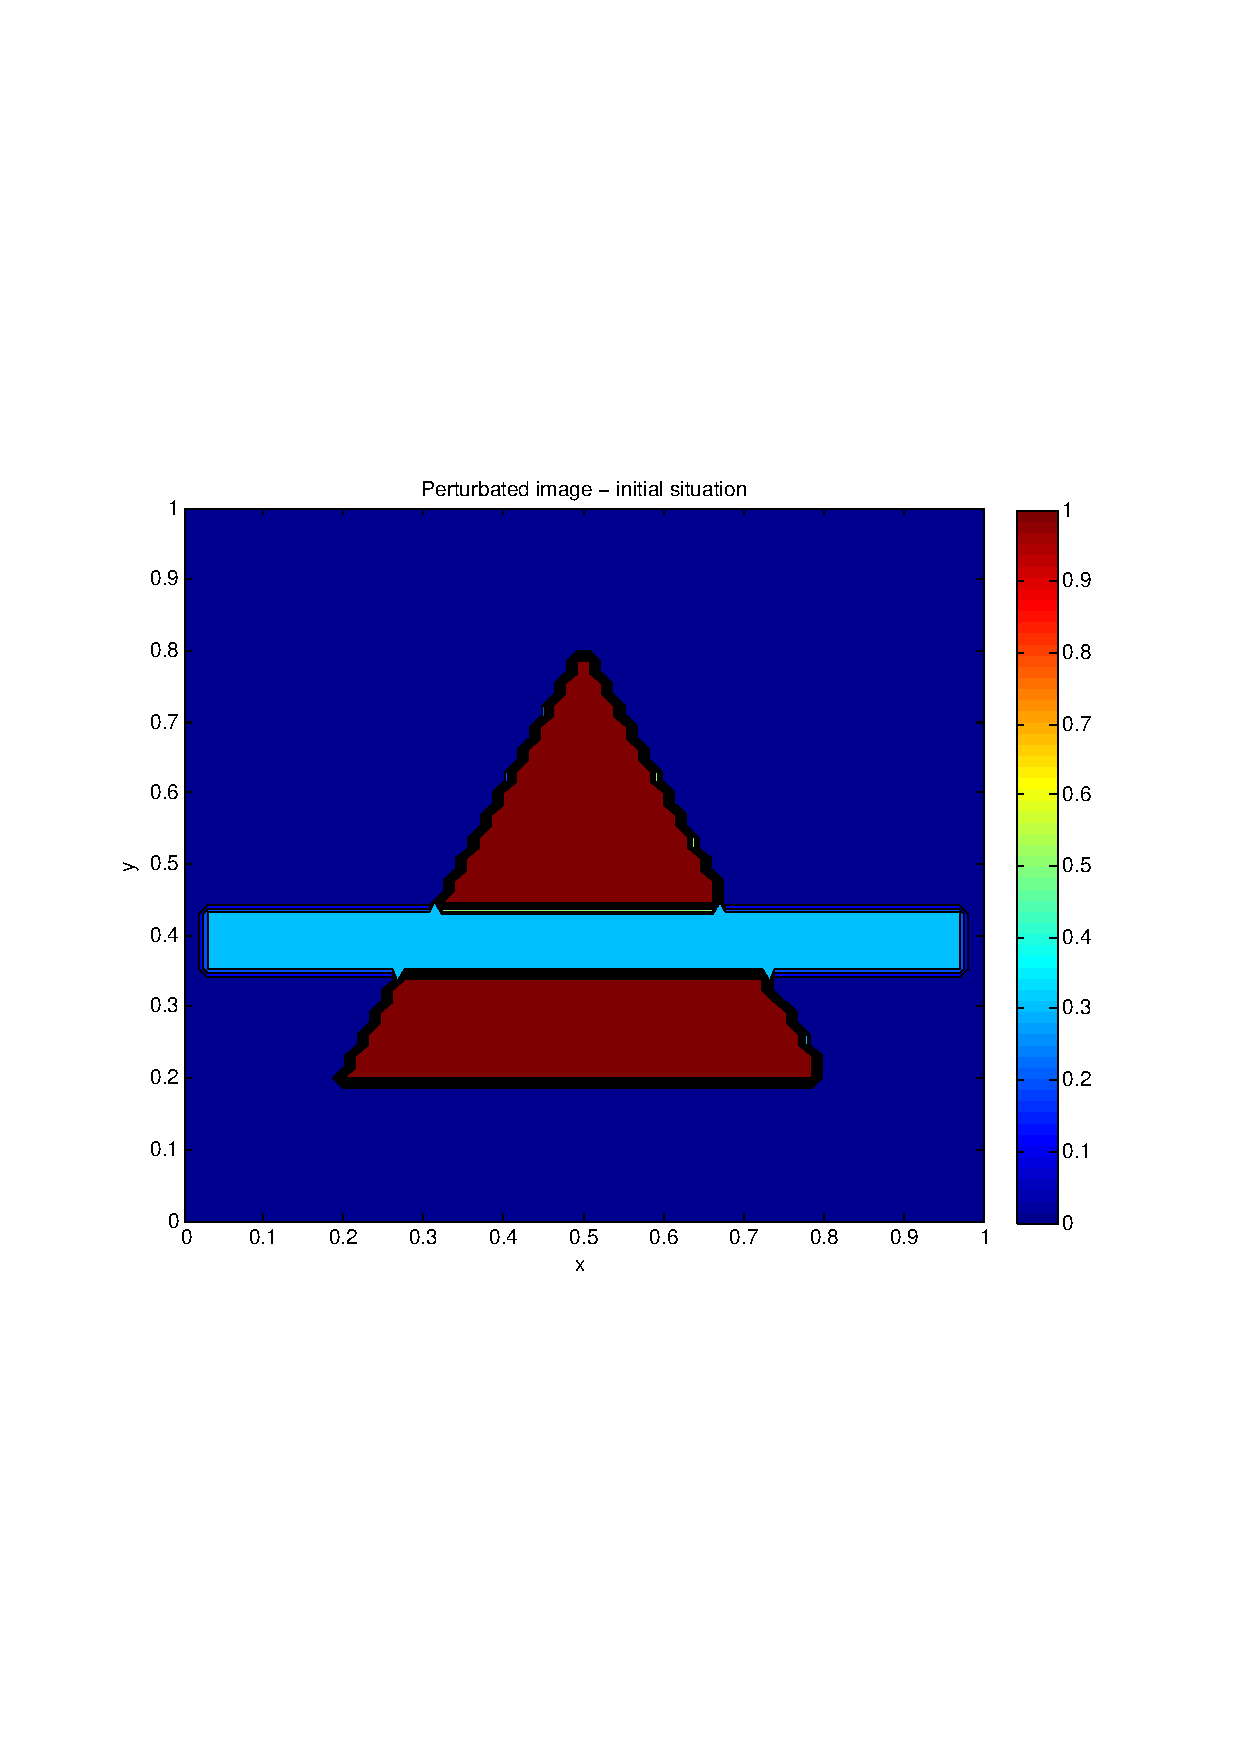
\includegraphics[width=11cm,height=15cm]{triangle_N_64_initial.pdf}
\end{center}
\vskip -3.cm
\caption{Inpainting with C-H. $\Delta t=0.001$, $\epsilon=0.05$, $N=64$ - Initial inpainted image}
\label{}
\end{figure}
\end{frame}
%%%%%%%%%%%%%%%%%%%%%%%%%%%%%%%%%%%%%%%%%%%%
 %Numerical results
 %%%%%%%%%%%%%%%%%%%%%%%%%%%%%%%%%%%%%%%%%%%%
\begin{frame}
\begin{figure}[!h]
\vskip -1.5cm
\begin{center}
\includegraphics[width=6.2cm,height=6cm]{triangle_Tfinal_N_64_DT_0p001.eps}
\includegraphics[width=6.2cm,height=6cm]{RSS_triangle_Tfinal_N_64_DT_0p001.eps}
\end{center}
\vskip -.5cm
\caption{Inpainting with C-H. $\Delta t=0.001$, $\epsilon=0.05$, $N=64$ - Restored triangle at $T=0.1$, classical (left) RSS method (right)}
\label{}
\end{figure}
\end{frame}
%%%%%%%%%%%%%%%%%%%%%%%%%%%%%%%%%%%%%%%%%%%%
 %Numerical results
 %%%%%%%%%%%%%%%%%%%%%%%%%%%%%%%%%%%%%%%%%%%%
 \begin{frame}
\begin{figure}[!h]
\vskip -1.5cm
\begin{center}
\includegraphics[width=6.2cm,height=6cm]{triangle_final_N_64_DT_0p001.eps}
\includegraphics[width=6.2cm,height=6cm]{RSS_triangle_final_N_64_DT_0p001.eps}
\end{center}
\vskip -.5cm
\caption{Inpainting with C-H. $\Delta t=0.001$, $\epsilon=0.05$, $N=64$ - Restored triangle with tresholding at $T=0.1$, classical (left) RSS method (right)}
\label{}
\end{figure}
\end{frame}

%%%%%%%%%%%%%%%%%%%%%%%%%%%%%%%%%%%%%%%%%%%%
 %Numerical results
 %%%%%%%%%%%%%%%%%%%%%%%%%%%%%%%%%%%%%%%%%%%%
 \begin{frame}
 {\small
 \begin{table}[!h]
\begin{center}
\begin{tabular}{|c|c||c|c|c|c|c|c|}
\hline 
Method& N & $\epsilon$ &  $\Delta t$& $\tau$  & $[0,T]$&quality &CPU factor (iterations)\\
 \hline
 RSS&$N=64$ & $0.05$ &  $10^{-3}$ & $1.4$  & $[0,0.1]$  & EX&12.86\\
 \hline
 Classic &$N=64$ & $0.05$ &  $10^{-3}$ & & $[0,0.1]$ &   EX&541.37\\
 \hline
 RSS&$N=64$ & $0.05$ &  $5.10^{-3}$ & $1.5$  & $[0,0.1]$  &EX&2.68\\
 \hline
 Classic &$N=64$ & $0.05$ &  $5.10^{-3}$ & & $[0,0.1]$ &   EX& 115.5\\
 \hline
 RSS&$N=64$ & $0.05$ &  $10^{-2}$ & $2.8$  & $[0,0.1]$  &middle&1.42\\
 \hline
 Classic &$N=64$ & $0.5$ &  $10^{-2}$ & & $[0,0.1]$ & middle &60.42\\
 \hline
 \hline
\end{tabular} 
\caption{2D Cahn-Hilliard Inpainting equation, the triangle example: , $\Omega=[0,1]^2$, $\lambda=90000$}
\label{AC_3D}
\end{center}
\end{table}
} 
 \end{frame}
 %%%%%%%%%%%%%%%%%%%%%%%%%%%%%%%%%%%%%%%%%%%%
 %Conclusion
 %%%%%%%%%%%%%%%%%%%%%%%%%%%%%%%%%%%%%%%%%%%%
 \section{Concluding Remarks}
 \begin{frame}
 \begin{itemize}
 \item RSS approach for parabolic equations present a compromise for preserving the stability of (semi)-implicit time schemes while simplifying the solution a each time step. 
 \item Versatility: possibility to apply the technique to a large number of times schemes
 \pause
 \item Main issue: saving computational time for a comparable precision
 \item Adaptive versions by varying $\tau$ at each iterations
 \item Limitation to parabolic equations: RSS does not apply interestingly, e.g.,  to Airy equation then not to KdV.
 \end{itemize}
 \end{frame}
 %%%%%%%%%%%%%%%%%%%%%%%%%%%%%%%%%%%%%%%%%%%%
 %
 %%%%%%%%%%%%%%%%%%%%%%%%%%%%%%%%%%%%%%%%%%%%
 \begin{frame}[allowframebreaks]
	\frametitle{References}
	\bibliographystyle{alpha}
	\bibliography{biblio}	
	\nocite{*}
\end{frame}

\end{document}